\section{Black Hole Fundamental Plane in Illustris}
\label{sec:analysis} To better understand the role of AGN in galaxy
evolution, we turn to large scale simulations with detailed gas physics
and energy transport like those found in the Illustris simulation. To analyze the black hole feedback physics in
the Illustris simulation, we attempt to reconstruct the black
hole fundamental plane from M03. Starting with our sample of black
holes from Section \ref{sec:sample}, we apply several models of a
accretion mechanisms to parametrized the components of the fundamental plane.

The fundamental plane from M03
is shown in Figure \ref{fig:Fp} and defined as

\begin{equation}
\log L_{R}=0.6\log L_{x}+0.78\log M_{BH}+7.33
\end{equation}
where the $L_{R}$ is the radio luminosity, $L_{X}$ is the X-ray
luminosity, and $M_{BH}$ is the mass of the black hole. This
expression, derived from empirical observations of accreting black holes with
masses ranging from $10-10^{9}M_{\odot}$, correlates the energy
output from the black hole with its mass. Another way to parametrize
the fundamental plane is using the mass, accretion rate, and X-ray
luminosity which is given by

\begin{equation}
\log L_{x}=\log M+q\log\dot{M}+K\;
\label{eq:LxFP}
\end{equation}
where $K$ is a normalization constant and $q$ reflects the efficiency
of the accretion mechanism. In M03, a range of $q$ values are given 
from 0.5 (optically-thick thin disk) to 2.3 (advection dominated
accretion flow) depending on the assumed accretion physics. 

\begin{figure}
\centering{}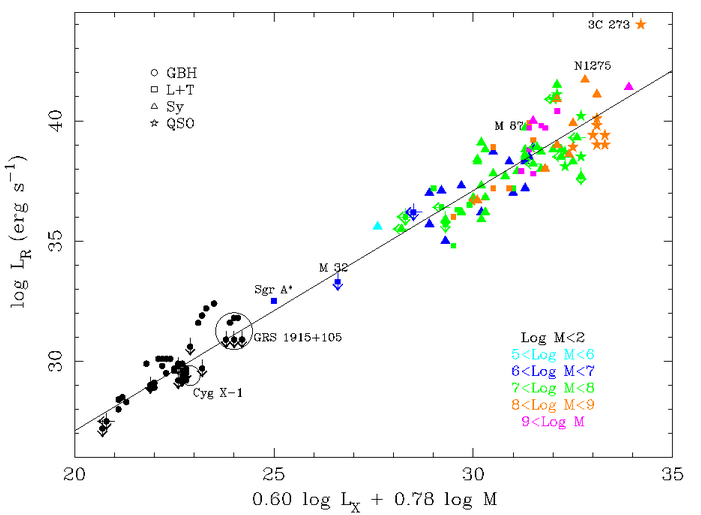
\includegraphics[clip,scale=0.35]{Figures/FP} \protect\caption{\label{fig:Fp}Edge-on view of the fundamental plane from M03 relating
the black hole mass to the radio and X-ray luminosities. Symbols indicate
the type of emission-line galaxy of the host and colors correspond
to the mass of the black hole in units of $\log\left({\rm M}_{\odot}\right)$.
Several well-known galaxies hosting an AGN are listed, as well.}
\end{figure}




Since luminosities are not calculated in any band in the Illustris
simulation, and since the black hole fundamental plane (Equation
\ref{eq:LxFP}) is expressed in terms of X-ray luminosity, we must
express the X-ray luminosity in terms of the quantities provided in
the simulation, black hole mass and accretion
rate. For the sake of variety, we will consider two models.
The first assumes a spherically-symmetric and symmetrically-accreting
mass surrounding the black hole:

\begin{equation}
L_{bol}=3.2\times10^3M \;.
\label{eq:Lbol_propto_m}
\end{equation}

The second assumes an optically-thick thin disk of material surrounding the black hole:

\begin{equation}
L_{bol}=4.648\times10^{19}\dot{M} \;.
\label{eq:Lbol_propto_dotm}
\end{equation}

Both of these approaches for the luminosity give the bolometric
luminosity. To get the X-ray luminosity from the bolometric luminosity
we use the \citet{elvis1994atlasof} data sample as a template.  The
template relates the bolometric luminosity and the X-ray 47 BH. The data are fit using a power
law given by Figure \ref{fig:Elvis_template}:

\begin{equation}
L_{x}=0.866L_{bol}+0.215\;.
\end{equation}

Considering the BHs have luminosity given by the Eddington luminosity with an efficiency of 10\% Eddington.  The 10\% efficiency is a general condition found in BH \textbf[{REFERENCE]}.  Using the Elvis Template the correlation between mass and bolumetic luminosity can be changed to mass and X-ray luminosity given by:

\begin{equation}
L_{x}=2.77E3M+ 0.215 \;.\label{eq:Lx_propto_m}
\end{equation}

The second model consider the luminosity mechanism to be proportional
to a thin disk accretion. For this case the efficiency is allso  10\% and that will be the case use in all the BH.  The thin disk luminosity relates the luminosity to the accretion rate.  Using the Elvis template the X-ray luminosity is express in terms of the accretion rate by:

\begin{equation}
L_{x}=4.02E19\dot{M}+ 0.215  \;,\label{eq:Lx_propto_mdot}
\end{equation}

for all the cases the masses, accretion rates and luminosities are
measured in $M_{\odot}$, $M_{\odot}s^{-1}$ and $L_{\odot}$. With
equations \ref{eq:Lx_propto_m} and \ref{eq:Lx_propto_mdot} and using
the equation \ref{eq:LxFP}. The fundamental plane equation can be
rewritten in terms of mass, accretion rate, k and q. 

To solve the equation we use the Levenberg-Marquard (NLLS)
algorithim.  For the thin-disk approximation $q = 0.3865\pm 0.0037$ and
$k = -4.425\pm 0.0465$.  For the Eddinton luminocity approximation $q = -0.0642\pm 0.0005$ and
$k = 20.107\pm 0.006$


\begin{figure}
\centering{}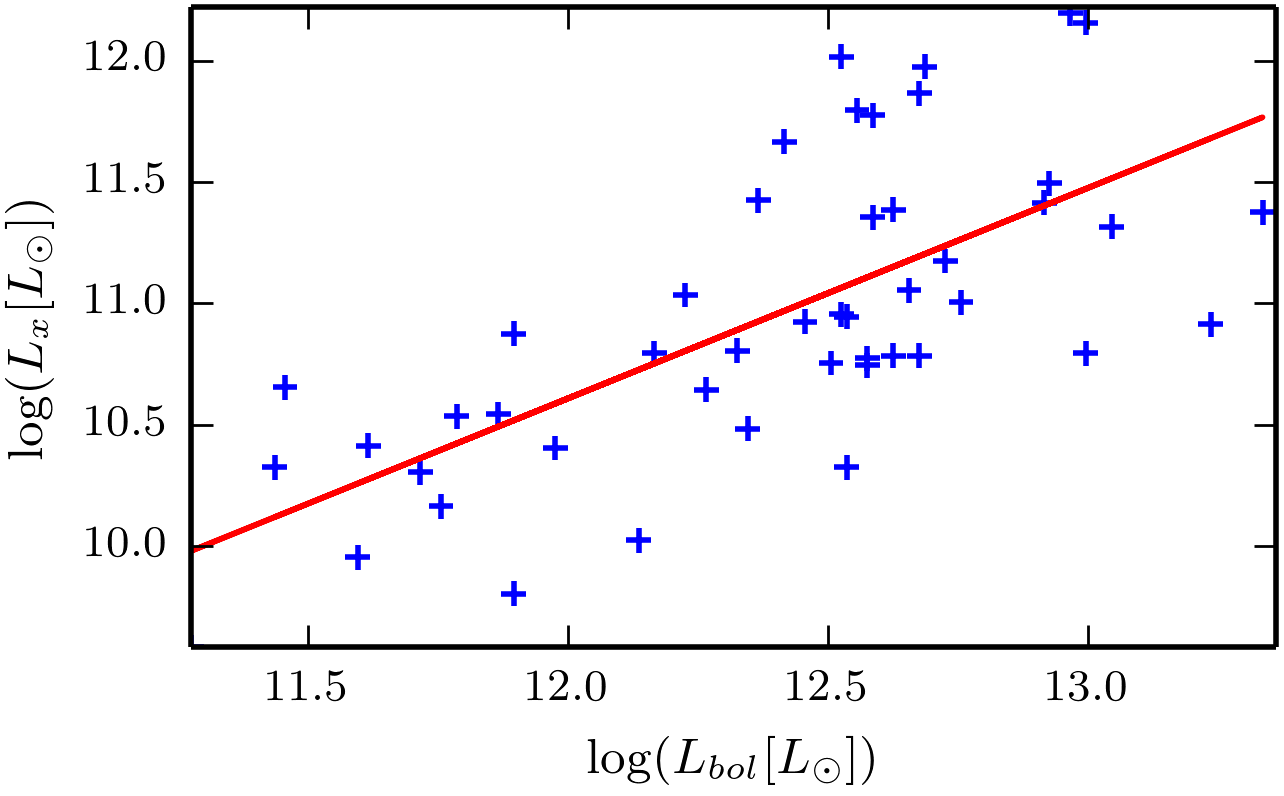
\includegraphics[clip]{Figures/elvis_template} \protect\caption{\label{fig:Elvis_template}The data points from the BH luminosities
over plot with the best-fit linear relation between $L_{x}$ and $L_{bol}$
for the sample.}
\end{figure}
\begin{figure}
\begin{centering}
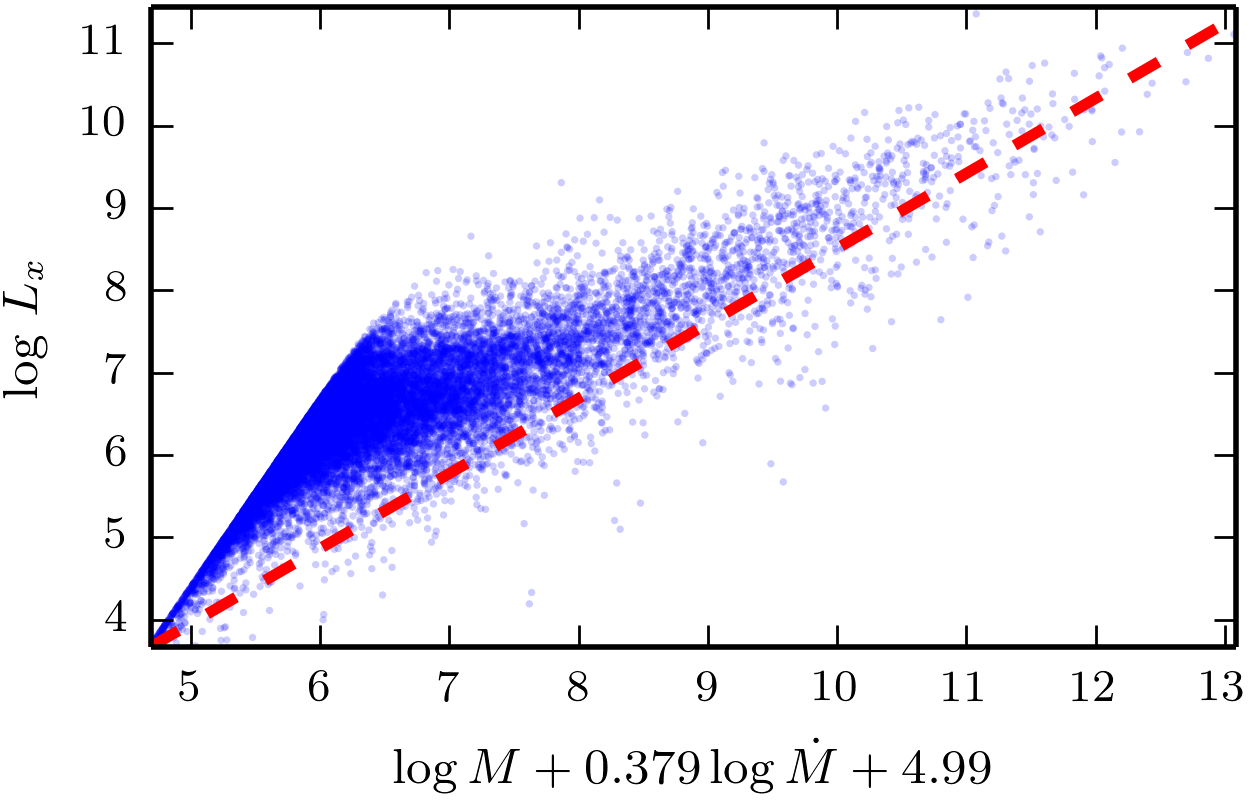
\includegraphics{Figures/fp_fit}
\par\end{centering}

\protect\caption{\label{fig:q_nr_hist}The fit to the fundamental plane
$\log\left(L_x\,[L_\odot]\right) = \log M+0.378\log\dot{{M}}+9.47$ using our sample. The
X-ray luminosities are in units of $L_\odot$, the masses in units of $M_\odot$, and the
accretion rate in units of $M_{\odot}\,s^{-1}$.}
\end{figure}


This relation allows us to construct a power-law
relationship between $M$ and $\dot{M}$ using linear least-squares
(Figure \ref{fig:bhpop_hist2d}). The best-fit is given by

\begin{equation}
\log\dot{M}=0.869\log M_{BH}-17.855.\label{eq:int_relation}
\end{equation}
This relationship reflects the intrinsic properties of the simulation,
and is independent of any models.


\begin{figure}
\centering{}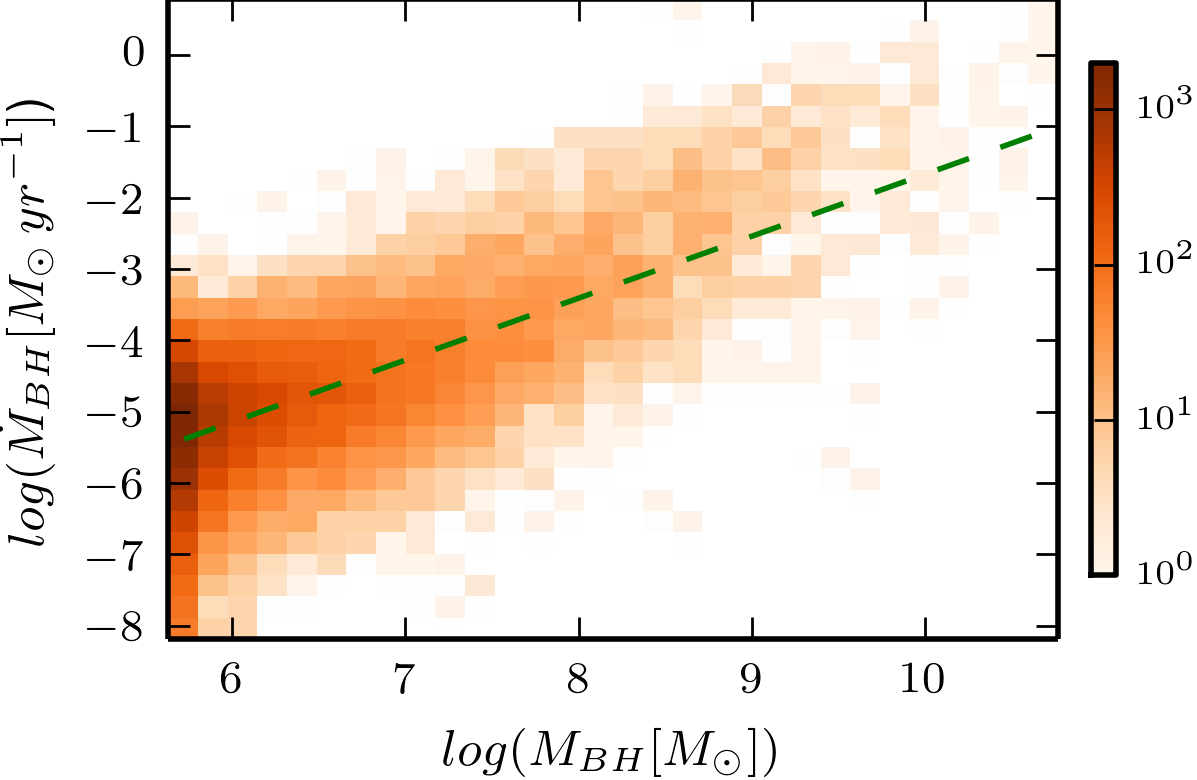
\includegraphics[clip]{Figures/Illustris2_bhpop_hist2d}
\protect\caption{\label{fig:bhpop_hist2d}Black hole accretion rate as a function of
black hole mass for the Illustrist-2 simulation for our sample. The
best-fit power-law relationship between $M$ and $\dot{M}$ is shown
in green. Colors correspond to a two-dimensional density of the same
plot sampled in log space.}
\end{figure}


From any accretion mechanism, we can calculate the bolometric
luminosity of the AGN. We use an empirical fit from 

To relate the X-ray luminosity with its bolometric luminosity from a particular accretion mechanism,
we use the Elvis template\citep{elvis1994atlasof}.
